% Prototype guide: everything about the code and the prototype of Investigate, Fix or Escalate.
% Build: ..\..\tools\tectonic.exe prototype_guide.tex   (or tectonic prototype_guide.tex)
% Written 10 November 2026 from the code as it stands (pilot model v2, settings v3, live demo).

\documentclass[11pt,a4paper]{article}

\usepackage[T1]{fontenc}
\usepackage{lmodern}
\usepackage[a4paper,left=2.2cm,right=2.2cm,top=2.2cm,bottom=2.4cm]{geometry}
\usepackage{amsmath}
\usepackage{enumitem}
\usepackage{booktabs}
\usepackage{tabularx}
\usepackage{longtable}
\usepackage{array}
\usepackage{float}
\usepackage{caption}
\usepackage{xcolor}
\usepackage{microtype}
\usepackage{fancyhdr}
\usepackage{tikz}
\usetikzlibrary{positioning,arrows.meta,fit,backgrounds}
\usepackage[hidelinks]{hyperref}

\setlength{\parindent}{0pt}
\setlength{\parskip}{5pt}
\setlist{leftmargin=1.5em, itemsep=2pt, topsep=2pt}
\captionsetup{font=small, labelfont=bf}
\newcolumntype{L}{>{\raggedright\arraybackslash}X}
\renewcommand{\arraystretch}{1.15}
\usepackage{url}
\makeatletter\g@addto@macro{\UrlBreaks}{\do\_\do\-\do\|\do\.\do\=}\makeatother
\newcommand{\file}[1]{{\small\path{#1}}}
\newcommand{\code}[1]{\path{#1}}

\definecolor{boxblue}{HTML}{C9DAF8}\definecolor{lineblue}{HTML}{6D8FC7}
\definecolor{boxpink}{HTML}{EBC6F3}\definecolor{linepink}{HTML}{A35DB5}
\definecolor{boxyel}{HTML}{FFE699}\definecolor{lineyel}{HTML}{BF9000}
\definecolor{boxgreen}{HTML}{C6E0B4}\definecolor{linegreen}{HTML}{548235}
\definecolor{note}{HTML}{F3F6FA}

\newsavebox{\kpbox}
\newenvironment{keypoint}{\par\smallskip\noindent\begin{lrbox}{\kpbox}\begin{minipage}{0.95\linewidth}}{\end{minipage}\end{lrbox}\fcolorbox{lineblue}{note}{\usebox{\kpbox}}\par\smallskip}

\pagestyle{fancy}
\fancyhf{}
\lhead{\small Prototype Guide}
\rhead{\small Opol Charis}
\cfoot{\small \thepage}
\renewcommand{\headrulewidth}{0.4pt}

\begin{document}

\begin{titlepage}
\centering
\vspace*{3cm}
{\LARGE\bfseries Investigate, Fix or Escalate\par}
\vspace{0.4cm}
{\Large The Prototype and its Code: A Complete Guide\par}
\vspace{1.2cm}
{\large Opol Charis\par}
{BSc Computer Science, Uganda Christian University\par}
\vspace{0.3cm}
{Department of Computing and Technology\par}
\vspace{1.5cm}
{10 November 2026\par}
\vfill
\begin{minipage}{0.85\linewidth}\small
This guide explains every part of the repository that the prototype depends on: the scenario
model, the simulator, the safety mechanism, the learning agent and its baselines, the
ticket-and-log readers, the triage loop, delegated checks, fix verification, the actions taken
after a decision, the live hidden-fault demo, the dashboards, the command line and the tests.
It describes the code as it stands on 10 November 2026 (pilot model v2, settings v3, agent
\file{v3_shielded_seed0}). All data are pilot data from one developer and fictional examples,
not Directorate data.
\end{minipage}
\vspace{1cm}
\end{titlepage}

\tableofcontents
\newpage

% =====================================================================================
\section{The prototype in one page}

\textbf{What it does.} The prototype takes an IT incident as people actually report it, a
helpdesk ticket in plain English plus an application log, and decides what to do with it. At
each step it can
\begin{enumerate}
  \item \textbf{investigate}: run one of 11 diagnostic checks (D01--D11),
  \item \textbf{fix}: apply the remedy for one of 8 causes (C01--C08), or
  \item \textbf{escalate}: hand the incident to a person.
\end{enumerate}
The decision is made by a \textbf{deep Q-network (DQN)} trained entirely in simulation. Every
proposal goes through an independent, rule-based \textbf{safety mechanism} first. A forbidden fix
is sent back to the agent once, and a second forbidden proposal in a row escalates the incident.
Every fix is then \textbf{verified}: a code change is tested on a staging copy of a repository,
and other remedies are judged by whether the symptoms clear. When the decision is final the
prototype \textbf{acts}. It opens a \emph{draft} pull request, writes a fix order to the owner,
or writes a routed escalation report. Nothing is merged and no message is really sent.

\textbf{The division of labour}, which is the most important design idea:
\begin{center}
\begin{tabularx}{\linewidth}{lL}
\toprule
Component & Its only job \\
\midrule
Reader (keywords or a language model) & Turns text into a fixed \emph{form}: symptoms, context, check results, each with a verbatim quote. It never names a cause or an action. \\
DQN agent & Chooses the next action from the form. It never sees the text. \\
Safety mechanism & Checks each proposed fix against the rules. It is not learnt, and the agent cannot change it. \\
Verifier & Says whether a fix cleared the symptoms. \\
Actions layer & Carries out the final, re-checked decision: a draft PR, a fix order or an escalation. \\
\bottomrule
\end{tabularx}
\end{center}

\begin{keypoint}
\textbf{One sentence for a viva:} a language model may \emph{read}, the trained agent
\emph{decides}, the rule checker \emph{permits}, staging tests \emph{verify}, and a person
\emph{merges}. No component does another's job.
\end{keypoint}

\textbf{Three ways in.}
\begin{itemize}
  \item \textbf{Command line:} \code{python -m src.prototype.cli --ticket ... --logs ...} (Section~\ref{sec:cli}).
  \item \textbf{Prototype dashboard} (Streamlit, port 8501): \file{dashboard/prototype_app.py}.
  \item \textbf{Live demo dashboard} (port 8502): \file{dashboard/live_app.py}, started by
        \file{run_live_demo.bat}. It shows incidents with hidden faults that nobody wrote by hand.
\end{itemize}

% =====================================================================================
\section{Architecture}

\begin{figure}[H]
\centering
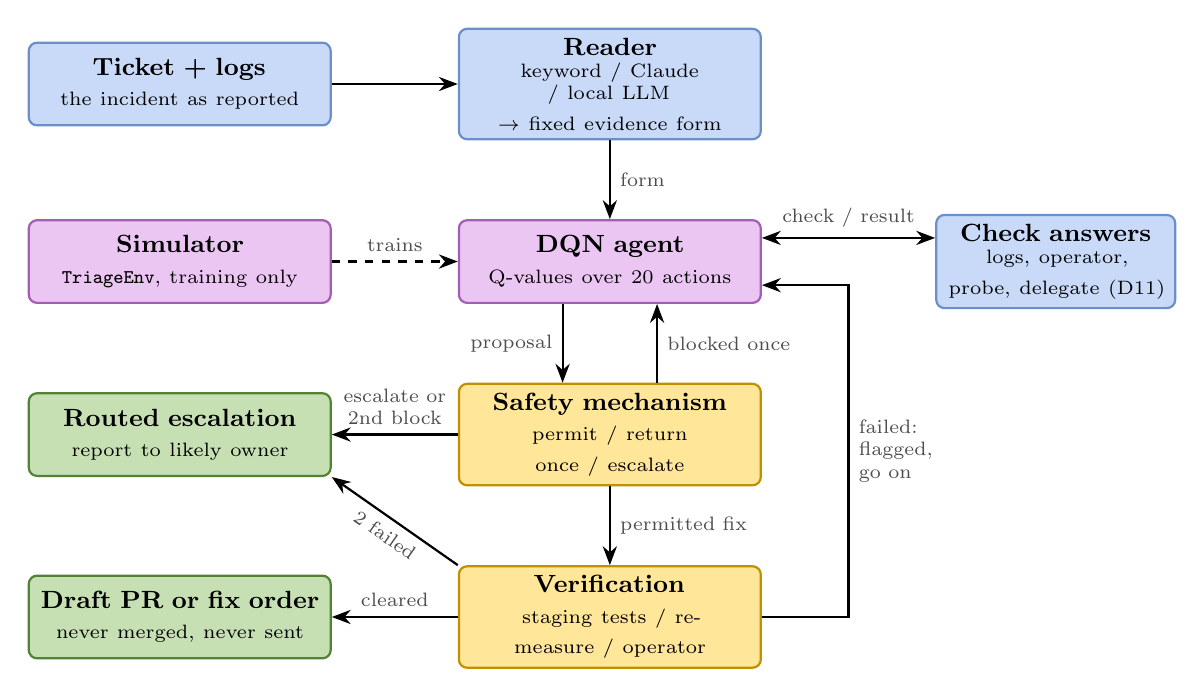
\begin{tikzpicture}[
  font=\small,
  box/.style={draw, rounded corners=3pt, align=center, minimum height=1.05cm, text width=3.6cm, line width=0.8pt},
  inp/.style={box, fill=boxblue, draw=lineblue},
  lrn/.style={box, fill=boxpink, draw=linepink},
  rul/.style={box, fill=boxyel, draw=lineyel},
  act/.style={box, fill=boxgreen, draw=linegreen},
  arr/.style={-{Stealth[length=2.4mm]}, line width=0.8pt},
  lab/.style={font=\scriptsize, text=black!70}]
\node[inp] (ticket) {\textbf{Ticket + logs}\\\scriptsize the incident as reported};
\node[inp, right=1.6cm of ticket] (reader) {\textbf{Reader}\\\scriptsize keyword / Claude / local LLM\\ $\to$ fixed evidence form};
\node[lrn, below=1.0cm of reader] (agent) {\textbf{DQN agent}\\\scriptsize Q-values over 20 actions};
\node[lrn, left=1.6cm of agent] (sim) {\textbf{Simulator}\\\scriptsize \texttt{TriageEnv}, training only};
\node[rul, below=1.0cm of agent] (safe) {\textbf{Safety mechanism}\\\scriptsize permit / return once / escalate};
\node[inp, right=2.2cm of agent, text width=2.8cm] (checks) {\textbf{Check answers}\\\scriptsize logs, operator,\\ probe, delegate (D11)};
\node[rul, below=1.0cm of safe] (ver) {\textbf{Verification}\\\scriptsize staging tests / re-measure / operator};
\node[act, left=1.6cm of safe] (esc) {\textbf{Routed escalation}\\\scriptsize report to likely owner};
\node[act, left=1.6cm of ver] (pr) {\textbf{Draft PR or fix order}\\\scriptsize never merged, never sent};
\draw[arr] (ticket) -- (reader);
\draw[arr] (reader) -- node[lab, right]{form} (agent);
\draw[arr, dashed] (sim) -- node[lab, above]{trains} (agent);
\draw[arr] ([xshift=-6mm]agent.south) -- node[lab, left]{proposal} ([xshift=-6mm]safe.north);
\draw[arr] ([xshift=6mm]safe.north) -- node[lab, right]{blocked once} ([xshift=6mm]agent.south);
\draw[{Stealth[length=2.4mm]}-{Stealth[length=2.4mm]}, line width=0.8pt] ([yshift=3mm]agent.east) -- node[lab, above]{check / result} ([yshift=3mm]agent.east -| checks.west);
\draw[arr] (safe) -- node[lab, above, align=center]{escalate or\\ 2nd block} (esc);
\draw[arr] (safe) -- node[lab, right]{permitted fix} (ver);
\draw[arr] (ver) -- node[lab, above]{cleared} (pr);
\draw[arr] (ver.north west) -- node[lab, sloped, below]{2 failed} (esc.south east);
\draw[arr] (ver.east) -- ++(1.1,0) |- node[lab, pos=0.25, right, align=left]{failed:\\ flagged,\\ go on} ([yshift=-3mm]agent.east);
\end{tikzpicture}
\caption{The prototype pipeline. Blue: input and evidence; pink: learning; yellow: rules and
verification; green: what happens afterwards. The simulator is used only for training; at run
time the same environment class is fed by the reader instead (\texttt{LiveTriageEnv}).}
\end{figure}

The key engineering decision is that the \emph{same} environment, observation, action mask,
safety mechanism and network are used in training, in evaluation and in the prototype. The
prototype replaces only the source of evidence. In training a random incident is drawn from the
scenario model. In the prototype the symptoms and context come from the reader, and a check's
result is looked up only when the agent asks for it (\code{LiveTriageEnv} in
\file{src/prototype/triage.py}).

% =====================================================================================
\section{Repository map}

\begin{longtable}{@{}p{5.6cm}p{9.9cm}@{}}
\toprule
Path & What it is \\
\midrule
\endhead
\multicolumn{2}{@{}l}{\textbf{Core study (simulation, rules, agents)}}\\
\file{src/sim/load_model.py} & Reads an elicitation workbook (.xlsx) into the scenario-model JSON. Provenance (\code{--rater}) is passed in, so no name reaches the JSON. \\
\file{src/sim/scenario.py} & \code{Scenario} dataclass and \code{build_scenario}: turns model + settings into arrays (likelihoods, prior, costs, rules, verification). \\
\file{src/sim/triage_env.py} & \code{TriageEnv}, the Gymnasium environment: one episode is one incident; also \code{Layout} to decode observations. \\
\file{src/rules/safety.py} & \code{RuleChecker}, \code{SafetyMechanism} (enforces), \code{RuleMonitor} (records only, optional penalty). \\
\file{src/agents/dqn.py} & Masked DQN (Stable-Baselines3 subclass), wrappers, hyperparameters, \code{AgentPolicy}. \\
\file{src/agents/baselines.py} & Always escalate, initial-symptom, scripted checklist, threshold policies. \\
\file{src/agents/belief.py} & Bayesian posterior over causes and expected information gain. \\
\file{src/agents/exact.py} & Exact optimal policy by dynamic programming (v1 settings only). \\
\file{src/agents/monitoring.py} & Training callback: scores the greedy agent every $N$ steps, writes \file{metrics.jsonl}, saves checkpoints. \\
\file{src/evaluation.py} & Runs a policy on fixed seeds and computes every Chapter 3 measure. \\
\multicolumn{2}{@{}l}{\textbf{Prototype}}\\
\file{src/prototype/reading.py} & \code{Finding}, \code{Reading}, the offline \code{KeywordReader}. \\
\file{src/prototype/llm.py} & \code{ClaudeReader}: schema-constrained form, redaction, quote check. \\
\file{src/prototype/local_llm.py} & Free local model via Ollama: \code{LocalReader}, \code{HybridReader}, \code{LocalDelegate}. \\
\file{src/prototype/delegate.py} & Delegated check D11: \code{ClaudeDelegate}, \code{PatternDelegate}. \\
\file{src/prototype/triage.py} & \code{LiveTriageEnv} and \code{triage()}, the decision loop and its report. \\
\file{src/prototype/verify.py} & Fix verification: staging tests, operator answer, demo case answer. \\
\file{src/prototype/actions.py} & Routing, handover reports, draft pull requests, simulated outbox. \\
\file{src/prototype/live.py} & Live hidden-fault incidents: draws, writes ticket and log, probes, re-measures, scores. \\
\file{src/prototype/cli.py} & Command line. \\
\multicolumn{2}{@{}l}{\textbf{Data, configuration and examples}}\\
\file{experiments/pilot/pilot_model_v2.json} & The scenario model the prototype uses (8 causes, 11 checks, 4 symptoms, 2 context attributes, 5 rules). \\
\file{experiments/pilot/pilot_settings_v3.json} & Researcher settings: rewards, check minutes, priors, noise, verification. \\
\file{experiments/pilot/prototype_config.json} & Which model, settings and agent run to use; reader keywords, log patterns and thresholds; context defaults; action settings. \\
\file{prototype/examples/} & Eight fictional cases (ticket, logs, optional \file{verification.json}) and \file{cases.json} with the intended cause and expected reading. \\
\file{prototype/toy_repo/} & Fictional student portal with four planted bugs (one per code-fault cause) and its tests. \\
\file{prototype/toy_repo_fixes/} & The pre-written fix and explanation for each planted bug. \\
\file{results/pilot/runs/} & One folder per training run: \file{config.json}, \file{metrics.jsonl}, \file{final.zip}. \\
\file{results/pilot/outbox/} & Simulated messages written by the actions layer. \\
\multicolumn{2}{@{}l}{\textbf{Interfaces and tests}}\\
\file{dashboard/app.py} & Training dashboard: training curves, the agent's ``thinking'', early prototype page. \\
\file{dashboard/prototype_app.py} & Full prototype dashboard (seven tabs). \\
\file{dashboard/live_app.py} & Live demo dashboard (Live incident and Stress test only). \\
\file{run_live_demo.bat} & Starts the live demo on port 8502. \\
\file{tests/} & 212 tests (Section~\ref{sec:tests}). \\
\bottomrule
\end{longtable}

% =====================================================================================
\section{The scenario model}\label{sec:model}

Everything the agent knows about the world comes from the \emph{scenario model}, a JSON file
read from an elicitation workbook (\file{src/sim/load_model.py}). The pilot model v2 was rated by
one software developer with three years' experience. It is not Directorate data.

\subsection{Causes}

\begin{center}\small
\begin{tabularx}{\linewidth}{@{}llLlll@{}}
\toprule
ID & Category & Cause & Freq. & Code fault & Owner \\
\midrule
C01 & Infrastructure & Slow external service, outbound call has no timeout & Occasional & yes & Integrations dev. \\
C02 & Database & Long-running transaction holds row locks & Common & no & DBA \\
C03 & Database & Missing index on a growing table & Rare & no & DBA \\
C04 & Application & Repeated queries per request (N+1) & Common & yes & Backend lead \\
C05 & Infrastructure & Cache failing silently, every request recomputes & Rare & yes & Backend lead \\
C06 & Application & Bad release or migration breaks a code path & Occasional & no & Release manager \\
C07 & Database & Duplicate rows where one was expected & Common & no & DBA \\
C08 & Authentication & Sign-in writes collide on the user row & Common & yes & Identity lead \\
\bottomrule
\end{tabularx}
\end{center}
Remedies: C01 set a timeout; C02 kill the blocking transaction; C03 add the index; C04 batch the
queries; C05 fix the cache serialisation; C06 roll back the release; C07 remove the duplicates;
C08 move the token write off the sign-in path. ``Code fault'' causes are fixed by a code change,
so the prototype can open a draft pull request for them.

\subsection{Checks, symptoms and context}

\begin{center}\small
\begin{tabular}{@{}lll@{\hspace{1.5em}}lll@{}}
\toprule
ID & Check & Effort & ID & Check & Effort\\
\midrule
D01 & Long outbound span in traces & Low & D07 & Query count in a slow trace & Medium\\
D02 & Lock-wait errors in logs & Low & D08 & Cache errors in logs & Low\\
D03 & DB connection pool usage & Low & D09 & Recent release or migration & Low\\
D04 & API node CPU & Low & D10 & Failure scope & Medium\\
D05 & Long transaction in the DB & Medium & D11 & Full log analysis (\emph{delegated}) & High\\
D06 & Query plan of slowest query & High & & & \\
\bottomrule
\end{tabular}
\end{center}

\textbf{Symptoms:} S01 server error on a page; S02 pages slow or timing out; S03 users can't sign
in or get logged out; S04 a save or approval fails after a long wait.
\textbf{Context:} X01 ``affected system is production'' (Yes/No); X02 priority (Low/Medium/High).

The model also holds two likelihood matrices, rated on a verbal scale and converted to
probabilities: $\theta_{ij} = P(\text{check } i \text{ positive}\mid\text{cause } j)$ and
$P(\text{symptom } i \text{ present}\mid\text{cause } j)$.

\subsection{Operational rules}

Each rule forbids one cause's remedy in a context \emph{unless} a named check has been observed:

\begin{center}\small
\begin{tabularx}{\linewidth}{@{}lllL@{}}
\toprule
Rule & Forbids fix for & When & Unless observed / reason \\
\midrule
R01 & C02 kill transaction & production & D05. Killing the wrong transaction rolls back valid work. \\
R02 & C06 roll back & production & D09. A rollback restarts every node; migrations may not reverse. \\
R03 & C07 remove duplicates & production & D10. Other records may depend on the rows; deletes are hard to undo. \\
R04 & C03 add index & priority High & D06. Index builds on large tables can block live traffic. \\
R05 & C01 set timeout & production & D01. A wrong timeout can make failures look like real results. \\
\bottomrule
\end{tabularx}
\end{center}

\subsection{Settings (v3, fix with verification)}

Settings are set by the researcher, not elicited (\file{pilot_settings_v3.json}). Rewards are in
hours (unit 60 minutes):
\begin{itemize}
  \item check cost: Low 5, Medium 15, High 30 minutes;
  \item escalation $c_{\text{esc}} = 120$ min $= 2$ h (elicited); correct fix reward $+5$;
  \item prior from frequency weights Rare 1, Occasional 2, Common 4;
  \item context: production 80\%; priority Low 30\%, Medium 50\%, High 20\%;
  \item $p_{\text{noise}} = 0.1$ (a check result is reversed), $p_{\text{miss}} = 0$, step limit 15;
  \item verification: each remedy has an apply time and a harm weight. Mean harm of a wrong fix
        $= (\text{wrong\_fix\_multiple} - 1)\times c_{\text{esc}} = 4 \times 2 = 8$ h, spread by harm
        weights (C07 2.0, C02 and C06 1.5, C03 1.0, C01 0.75, code faults 0.5). After
        \textbf{2 failed fixes} a person takes over.
\end{itemize}
\code{build_scenario} validates all of this: rewards must satisfy
correct $>$ $-$escalate $>$ $-$wrong, every frequency and effort must have a value, context
probabilities must sum to one, and with verification a correct fix must beat escalation for
every remedy. An optional \emph{overlap} $\omega$ blends the likelihoods of causes in the same
category: $\theta'_{ij} = (1-\omega)\theta_{ij} + \omega\,\overline{\theta_{i\cdot}}$.

% =====================================================================================
\section{The simulator: \texorpdfstring{\texttt{TriageEnv}}{TriageEnv}}

\textbf{One episode is one incident.} At \code{reset(seed)} everything is drawn once, so the same
seed gives every policy the same incident:
\begin{enumerate}
  \item the hidden cause $j \sim$ prior; the context from its probabilities;
  \item the symptoms, each present with probability \code{symptom_theta[i, j]};
  \item each check's true result $\sim \theta_{ij}$, then reversed with probability $p_{\text{noise}}$;
  \item whether each check is available ($1-p_{\text{miss}}$).
\end{enumerate}

\textbf{Actions} (20 with model v2): 11 checks, 8 fixes and 1 escalation, in that order.

\textbf{Observation} (70 numbers, all in $[0,1]$):
\begin{itemize}
  \item each check's status one-hot over \{not requested, unavailable, negative, positive\} ($4\times11$);
  \item each symptom one-hot over \{present, absent, not reported\} ($3\times4$);
  \item context: one number for a two-valued attribute, one-hot otherwise ($1+3$);
  \item step count / max steps and a ``last proposal was blocked'' flag (2);
  \item with verification: one ``this fix was tried and failed'' flag per cause (8).
\end{itemize}
During training the 20-value action mask is appended, so the network sees 90 inputs.

\textbf{Action mask:} a check can be run only once; a failed fix cannot be repeated; a blocked
action is masked for the next step.

\textbf{Rewards and endings (v3):}
\begin{center}\small
\begin{tabularx}{\linewidth}{@{}lL@{}}
\toprule
Action & Effect \\
\midrule
Run check $i$ & $-$cost$_i$; the status becomes positive / negative / unavailable \\
Fix the true cause & $+5 - $ apply cost; episode ends \emph{correct} \\
Fix a wrong cause & $-($apply cost $+$ harm$)$; that fix is flagged and masked; after 2 failed fixes, also $-2$ and the episode ends \emph{fix\_limit} \\
Escalate & $-2$; ends \emph{escalated} \\
Step limit (15) & $-2$; ends \emph{step\_limit} (counted as an escalation) \\
\bottomrule
\end{tabularx}
\end{center}
Without verification (v1/v2) any fix ends the episode, correct ($+5$) or wrong ($-10$).

\textbf{Reference label} (evaluation only, never shown to the agent): an incident ``should be
escalated'' if a rule would block the true cause's fix with no lifting check available, or if
even the full evidence points to a different cause. This label drives the escalation precision,
recall and MCC.

% =====================================================================================
\section{The safety mechanism}

\file{src/rules/safety.py} is deliberately separate from both the agent and the environment.
\begin{itemize}
  \item \code{RuleChecker.forbidding(action, context, observed)} returns the rules that forbid an
        action now. Only fixes can be forbidden; checks and escalation are always allowed. A rule is
        lifted once its \code{unless_observed} check has returned a result (``unavailable'' does not count).
  \item \code{SafetyMechanism} (the \emph{shielded} agent): a permitted proposal passes unchanged.
        The first refusal uses a step with no reward, sets the blocked flag and masks that action.
        A second refusal in a row calls \code{force_escalation()}. \textbf{No prohibited action ever
        reaches the environment.}
  \item \code{RuleMonitor}: lets everything through and only counts violations. With
        \code{penalty=10} it subtracts 10 per violation, which gives the \emph{penalty-only} agent.
        With no penalty it is the \emph{unconstrained} agent.
\end{itemize}
In the prototype the rule checker is used a \emph{second} time on the final decision with the
final evidence (\code{decision["permitted"]}), and \file{actions.py} refuses to act unless this
is \code{True}.

% =====================================================================================
\section{The agents}

\subsection{Masked DQN}
\file{src/agents/dqn.py} subclasses Stable-Baselines3's DQN:
\begin{itemize}
  \item \code{MaskInObservation} appends the action mask to the observation, and
        \code{MaskedQNetwork} sets masked Q-values to $-10^9$. Masking therefore covers both action
        choice and the $\max$ in the learning target.
  \item \textbf{Masked exploration with a check bias:} random actions respect the mask, and 80\% of
        them are checks, so exploration reaches long investigations.
  \item Optional \textbf{Double DQN} target (online network picks, target network values), which
        the v3 runs use.
  \item Rewards are divided by 10 during training only (\code{ScaleReward}); \code{q_values()}
        returns them unscaled, in hours.
\end{itemize}
\textbf{Hyperparameters of the prototype's agent} (\file{results/pilot/runs/v3_shielded_seed0}):
500,000 steps, network $2\times128$, learning rate $10^{-4}$, buffer 200,000, batch 64,
$\gamma = 1$, target update every 1,000 steps, $\varepsilon$ from 1.0 to 0.05 over the first 30\%,
Double DQN on. Seed 0 of three was chosen on the training monitor's return, not on evaluation
incidents.

\subsection{Baselines and the exact policy}
\begin{itemize}
  \item \textbf{Always escalate.}
  \item \textbf{Initial-symptom:} fixes the most probable cause given the symptoms, with no checks.
  \item \textbf{Scripted ($k$):} runs a fixed list of $k$ checks ordered by average information
        gain, then fixes the most probable cause.
  \item \textbf{Threshold ($\tau$):} runs the most informative check until a permitted cause reaches
        probability $\tau$, then fixes it; escalates when the checks run out.
\end{itemize}
The baselines are given the likelihood model (Bayesian posterior, \file{belief.py}); the DQN is
not. \file{exact.py} solves the v1 problem exactly by dynamic programming over all
$3^{10}\times16\times6$ evidence states, giving the optimal value. It refuses missing checks and
verification.

\subsection{Training and evaluation}
\file{experiments/pilot/train_dqn.py} and \file{run_comparison.py} train the agents.
\code{TrainingMonitor} scores the greedy agent on 1,000 fixed incidents every 25,000 steps.
Seed ranges never overlap: training below $10^6$, evaluation from $10^6$, tuning from
$2\times10^6$, monitoring from $3\times10^6$. \code{summarise()} computes return (with bootstrap
CI), resolution accuracy, wrong-fix rates, checks and check cost, escalation
rate/precision/recall/F1/MCC, proposed and executed violation rates, forced escalations and
compliant success.

% =====================================================================================
\section{The prototype pipeline in detail}

\subsection{Readers: from text to a form}
A reader returns a \code{Reading}: category, one-line summary, and a \code{Finding} for every
symptom, context attribute and check. Each finding holds its \code{value}, the \code{evidence}
(the exact sentence or log line) and its \code{source} (ticket, logs, default, operator, probe,
delegate).

\begin{center}\small
\begin{tabularx}{\linewidth}{@{}lL@{}}
\toprule
Reader & How it works \\
\midrule
\code{keyword} & Offline. Keyword lists for the ticket; regular expressions with thresholds for the log (e.g.\ pool usage above 80\%), time windows (e.g.\ a release within 24 h of the newest line) and median/max aggregation. All patterns live in \file{prototype_config.json}. \\
\code{claude} & Claude fills a JSON form whose schema is built from the scenario model, so a new model needs no code change. The prompt forbids diagnosis. \\
\code{local} & \code{HybridReader}: a local model (Ollama, \code{qwen3:4b}) reads only the ticket; the keyword patterns read the log, where numbers against thresholds matter. Takes about 30--45 s. \\
\code{local-full} & \code{LocalReader} on both ticket and log, slower. It asks for a compact list form with one worked example, then converts it back to the full form. \\
\bottomrule
\end{tabularx}
\end{center}

\textbf{Safeguards on every language-model reader:}
(1) \emph{redaction} before sending: e-mails, secrets, IPs, Ugandan phone numbers and long tokens
become placeholders; (2) \emph{schema-constrained output}, so the model cannot propose a fix;
(3) the \emph{quote check}: a finding whose quote is not in the (redacted) ticket or log is
discarded with a warning, so an invented line cannot become evidence; (4) ticket text is
declared to be data, not instructions.

\textbf{Defaults:} unstated context takes the stricter value (production, High priority), since
both switch rules on. An unmentioned symptom counts as absent, as in training.

\subsection{The triage loop}
\texttt{triage(reading, scenario, model, agent, ask, delegate, ticket, logs, verify)}:
\begin{enumerate}
  \item builds the symptom and context vectors from the reading, and resets the live environment
        wrapped in the safety mechanism, \texttt{SafetyMechanism(LiveTriageEnv(...))};
  \item at each step computes the agent's Q-values and takes the greedy action;
  \item a \textbf{check} is answered lazily by \code{lookup}. A delegated check (D11) goes to the
        delegate. Otherwise the reading's finding is used. If the logs did not show it,
        \code{ask(check)} is called: the operator on the command line, or a \code{Probe} in
        live mode. With no answer the check is \emph{unavailable};
  \item a \textbf{fix} goes through the safety mechanism, then the verifier. ``Cleared'' means
        resolved; ``not cleared'' flags the fix as failed and the agent continues; no answer
        stops the incident as \emph{awaiting verification};
  \item each step records the action, its Q-value, the margin over the runner-up, the top-3
        alternatives, the escalation value, the result and its evidence, any blocking rule, any
        verification, and the Bayesian belief over causes. The belief is \emph{for the viewer
        only}; the agent never sees it.
\end{enumerate}
The report holds the reading, the steps and the decision (outcome, checks run, minutes, blocked
proposals, attempts, cause, remedy, \code{permitted}, \code{verified}). It also gives the three
most probable causes, from the ratings, for whoever takes the incident next.

\subsection{Delegated check D11}
D11 ``full log analysis'' is an ordinary check marked \code{"delegated": true} with High cost.
When the agent picks it, a fixed prompt template, filled from the check's definition (the agent
does not write the prompt), is sent to a delegate (\code{claude}, \code{local}, or the offline
\code{pattern}). The answer is reduced to positive, negative or not shown plus a quote. Only that
result reaches the agent; the delegate's written report is kept for the person. The same
redaction and quote check apply. In the pilot D11 asks whether the stack traces point into the
application's own code (\file{portal/...}).

\subsection{Verification}
\file{src/prototype/verify.py} chains verifiers, and the first definite answer wins:
\begin{enumerate}
  \item \code{StagingVerifier} (code faults only): copies the toy repository to a temporary
        folder, applies the patch, and runs the tests. The patch must break no test that passed
        before, \emph{and} the incident's own reproduction tests (from \file{verification.json})
        must now pass. ``The patch passes some test'' is not enough, because all planted bugs are
        present at once.
  \item \code{AnswerVerifier}: the operator says whether the symptoms cleared.
  \item \code{CaseVerifier} (demo only, \code{--demo-verify}): the cause the example case was written to show.
\end{enumerate}
A verifier acts on nothing real. The patch that was verified is stored and is exactly the patch
the later pull request carries (\code{StoredPatcher}).

\subsection{Actions after the decision}
\file{src/prototype/actions.py} is a demo layer and is not part of the evaluated study.
\begin{itemize}
  \item \textbf{Routing:} a fix goes to the cause's owner. An escalation goes to the owner of the
        most probable cause if it reaches 50\%, otherwise to the fallback (senior developer).
  \item \textbf{Code fault $\to$ draft pull request} on the toy repository: local (a branch in
        \file{results/pilot/demo_repo}) or GitHub (one configured throwaway repository). The patch is
        pre-written or written by Claude, and the tests are re-run.
  \item \textbf{Other fix $\to$ fix order}; \textbf{escalation $\to$ handover report} with the
        ticket, every step and its evidence, the most probable causes and the fixes already tried.
  \item Messages are written to \file{results/pilot/outbox/}. Nothing is sent.
\end{itemize}
\textbf{Guarantees enforced in code:} (1) nothing acts unless \code{permitted} is true;
(2) PRs only for \code{code_fault} causes, and only as drafts; (3) a patch may only change an
existing non-test source file; (4) a command allow-list (\code{git init/add/commit/checkout/clone/push/config},
\code{gh pr create --draft}); pushing \code{main}/\code{master} or forcing is refused. Nothing
ever merges.

\subsection{Live mode: hidden-fault incidents}
\file{src/prototype/live.py} creates incidents that nobody wrote and nobody has seen:
\begin{itemize}
  \item \code{draw()} samples an incident exactly as the training environment does (cause, context,
        symptoms, check results with reversals). Three origins: \emph{random}, \emph{chosen}
        (someone plants the cause), or \emph{your ticket} (the reader's symptoms, context and stated
        results fix the hidden system, and the cause is drawn given them).
  \item \code{write_ticket()} and \code{write_logs()} turn it into text: a ticket from phrase
        banks (never naming the cause), and a log with background traffic, failing requests,
        evidence lines for about 55\% of checks (often \emph{near misses} below a threshold or
        outside a window), and stack traces for D11.
  \item \code{Probe} answers a check the log does not cover from the hidden system, with a
        realistic console command and its output.
  \item \code{Remeasure} verifies non-code fixes by ``re-measuring'' the symptoms: they clear only
        if the fix was for the hidden cause. Code faults go through the staging tests against the
        hidden fault's reproduction tests.
  \item At the reveal: the hidden cause, the outcome, which results were reversed by noise, the
        reader's mistakes, and \code{hindsight()}, the cause that \emph{all} check results together
        point to. When that is wrong, escalating was the sound choice.
\end{itemize}

\subsection{The local language model}
\file{local_llm.py} talks to Ollama at \code{http://localhost:11434} (model \code{qwen3:4b},
temperature 0, JSON-schema output), so nothing leaves the laptop. Environment variables
\code{TRIAGE_LLM_URL}, \code{TRIAGE_LLM_MODEL}, \code{TRIAGE_LLM_KEY} switch it to any
OpenAI-compatible endpoint. Use that only for fictional tickets, because the text then leaves
the machine.

% =====================================================================================
\section{Using the prototype}\label{sec:cli}

\subsection{Set-up}
\begin{verbatim}
python -m venv --system-site-packages .venv
.venv\Scripts\python -m pip install -r requirements.txt
winget install Ollama.Ollama        (optional, for the local reader)
ollama pull qwen3:4b
\end{verbatim}
The Claude reader needs \code{ANTHROPIC_API_KEY}. Use it only on fictional tickets unless the
Directorate approves.

\subsection{Command line}
\begin{verbatim}
python -m src.prototype.cli --ticket prototype\examples\sign_in\ticket.txt
       --logs prototype\examples\sign_in\logs.txt --act
\end{verbatim}
\begin{center}\small
\begin{tabularx}{\linewidth}{@{}lL@{}}
\toprule
Flag & Meaning \\
\midrule
\code{--reader keyword|local|local-full|claude} & Who reads the text (default keyword, offline). \\
\code{--ask} & Ask you for checks the logs do not show, and whether a fix cleared the symptoms. \\
\code{--delegate pattern|local|claude|off} & Who answers D11 (default pattern). \\
\code{--act} & Carry the decision out (draft PR, fix order or escalation report). \\
\code{--pr local|github|off}, \code{--patcher pre-written|claude} & Where PRs go and who writes the patch. \\
\code{--demo-verify} & Example cases only: verify against the intended cause. \\
\code{--run DIR}, \code{--json FILE}, \code{--incident ID} & Agent run, save the report, name the incident. \\
\bottomrule
\end{tabularx}
\end{center}

\subsection{Dashboards}
\textbf{Prototype dashboard} (\code{streamlit run dashboard/prototype_app.py}, port 8501), tabs:
\emph{Live incident}, \emph{Stress test}, \emph{Triage a ticket} (reading $\to$ steps $\to$
decision $\to$ verify $\to$ action, with the PR diff), \emph{All example cases},
\emph{Outbox and draft PRs}, and reader \emph{accuracy}. The sidebar chooses the agent run,
reader, delegate, actions, and how fixes are verified, and shows a green dot when the local model is ready.

\textbf{Live demo} (\file{run_live_demo.bat}, port 8502): only the Live incident and Stress test
tabs. The run sheet is \file{documentation/live_demo.md}:
\begin{enumerate}
  \item \emph{Random hidden fault}: new incident (padlock closed) $\to$ let the agent work (an animated
        console with the belief bars, blocks and verifications) $\to$ reveal (padlock opened).
  \item \emph{Someone plants the fault}: an audience member picks the cause.
  \item \emph{Your own ticket}: someone dictates a ticket; the local model reads it.
  \item \emph{Stress test}: 20--500 fresh incidents in seconds (keyword reader, re-measuring),
        showing resolved \%, first fix worked \%, escalations, and how many escalations were
        sound (the evidence itself pointed to the wrong cause).
\end{enumerate}

\textbf{Training dashboard} (\file{dashboard/app.py}): training curves of any run, and a
``thinking'' view that compares the agent's Q-values with the exact solution.

% =====================================================================================
\section{Tests}\label{sec:tests}
Run with \code{python -m pytest} (about five minutes). The table counts test functions; with parametrisation pytest collects 212 tests.
\begin{center}\small
\begin{tabularx}{\linewidth}{@{}lrL@{}}
\toprule
File & Functions & What it protects \\
\midrule
\file{test_load_model.py} & 12 & Workbook reading, rule conditions, likelihood grids \\
\file{test_triage_env.py} & 25 & Drawing, observations, masks, rewards, verification, step limit \\
\file{test_safety.py} & 26 & Block-then-escalate, rule lifting, monitor and penalty \\
\file{test_baselines.py} & 21 & Posterior, information gain, each baseline, exact solver \\
\file{test_dqn.py} & 10 & Masking in network and exploration, Double DQN target \\
\file{test_prototype.py} & 21 & Readers, redaction, quote check, triage loop on the examples \\
\file{test_extension.py} & 20 & Delegation, routing, draft PR guarantees, command allow-list \\
\file{test_verify.py} & 12 & Verification in the environment \\
\file{test_prototype_verify.py} & 8 & Staging verifier and verifier chain \\
\file{test_live.py} & 11 & Live draws reproducible; ticket and log never name the cause; probing; fixes verified only for the hidden cause; never a wrong fix; own-ticket mode; local reader and delegate forms \\
\midrule
Total & 166 & 212 tests once parametrised; all pass \\
\bottomrule
\end{tabularx}
\end{center}

% =====================================================================================
\section{Results so far}

\textbf{Simulation} (5,000 identical evaluation incidents, escalation 120 min, agents mean of 3
seeds; returns in hours):
\begin{center}\small
\begin{tabular}{@{}lrrrrrr@{}}
\toprule
Policy & Return & Resolved & Any wrong fix & Escalated & Checks & Rule broken \\
\midrule
Always escalate & $-2.00$ & 0.0\% & 0.0\% & 100.0\% & 0.00 & 0.0\% \\
Initial-symptom & $-2.33$ & 41.3\% & 28.6\% & 58.7\% & 0.00 & 0.0\% \\
Scripted ($k=9$) & $-1.38$ & 88.3\% & 29.7\% & 11.7\% & 9.00 & 0.0\% \\
Threshold ($\tau=0.65$) & $-0.38$ & 74.1\% & 21.4\% & 25.9\% & 4.72 & 0.0\% \\
DQN + safety mechanism & $-0.41$ & 67.6\% & 22.5\% & 32.4\% & 5.73 & 0.0\% \\
DQN unconstrained & $-0.28$ & 74.7\% & 24.9\% & 25.3\% & 6.05 & 7.6\% \\
DQN penalty-only & $-0.24$ & 74.7\% & 25.4\% & 25.3\% & 4.98 & 0.0\% \\
\bottomrule
\end{tabular}
\end{center}
Behind the mechanism, 0 of 15,000 agent incidents executed a rule violation. Proposals that
break a rule settle at 20--25\%, because a block costs nothing in the pilot. Escalation rises and
wrong fixes fall as the cost of escalation rises (60 / 120 / 240 min).

\textbf{Prototype} (eight fictional cases, keyword reader, agent v3): reading 100\% correct on
symptoms, context and checks. Six of eight cases end as intended: results\_approval, sign\_in,
transcript\_duplicates, class\_results\_slow and profile\_cache are fixed and verified, and
vague\_slow (written to have no cause) has a wrong guess that fails verification and is then
escalated. fees\_release (C06) and payment\_gateway (C01) are escalated instead of fixed. These
cases show that the pipeline works; they do not measure accuracy.

% =====================================================================================
\section{Limitations to state honestly}
\begin{itemize}
  \item One rater (a developer), not the Directorate; several values are set by the researcher,
        including all verification settings.
  \item Three seeds per agent (ten planned); only the base ambiguity level was run.
  \item A blocked proposal costs nothing, so the shielded agent leans on the mechanism.
  \item Verification is assumed reliable. In live mode it is perfect by construction.
  \item The keyword reader is tuned to the example log format; the live log is written in that
        same format. Live incidents come from the agent's own world (the scenario model), so they
        show that the pipeline works, not that the model fits real incidents.
  \item The toy repository, the outbox and the PRs are fictional; nothing touches a real system.
\end{itemize}

% =====================================================================================
\section{How to extend it}
\begin{itemize}
  \item \textbf{Directorate model:} fill the Directorate workbook, then run
        \texttt{python -m src.sim.load\_model WORKBOOK.xlsx model.json -{}-label ... -{}-rater "role"}.
        Add owners, \code{code_fault} and delegated flags. Point \file{prototype_config.json} at it,
        add keyword and pattern entries for each new symptom, context value and check, add
        verification settings for each remedy, and retrain. The Claude and local readers need no
        code change, because their form is built from the model.
  \item \textbf{A new check:} add it to the model (with likelihoods), give it a pattern in
        \code{checks} of the config (\code{covers}, \code{positive}, optional \code{above},
        \code{within_hours}, \code{aggregate}), and for live mode an evidence line in
        \code{_evidence_lines} and a probe command.
  \item \textbf{A new code-fault fix:} a bug in \file{prototype/toy_repo}, a failing test, the fix in
        \file{prototype/toy_repo_fixes/<cause>/}, and a case with \file{verification.json} naming
        the reproduction test.
\end{itemize}

% =====================================================================================
\section{Questions you are likely to be asked}
\begin{description}[style=nextline, leftmargin=1em]
  \item[Does the language model make the decision?] No. It only fills a fixed form, and its
        schema has no place for a cause or an action. The trained DQN decides.
  \item[What stops a hallucinated log line from becoming evidence?] The quote check discards any
        finding whose quote is not literally in the ticket or log.
  \item[Can the agent break a rule?] Not behind the mechanism: a forbidden fix never reaches the
        environment, and the final decision is checked again before anything acts.
  \item[Why does the shielded agent still propose forbidden fixes?] A block is free in the pilot.
        Charging for it is the planned ablation.
  \item[Why can't a wrong fix ``succeed''?] With verification the symptoms clear only for the
        right cause. A wrong fix is flagged, and the agent goes on or escalates after two.
  \item[Why did it escalate a case it could have fixed?] The value of escalating was higher
        given the evidence and the cost of a wrong, hard-to-undo remedy. The stress test also
        shows how many escalations were sound because the evidence itself pointed elsewhere.
  \item[Is any real data sent anywhere?] The keyword reader and Ollama run locally. The Claude
        reader redacts first and is for fictional tickets only. Messages go to a local outbox.
\end{description}

\end{document}
